\chapter{Attacchi TCP/IP}

\section{Livello di trasporto}
La responsabilità principale del livello di trasporto è la consegna 
dei dati da processo a processo. I singoli processi in esecuzione su un 
dato host sono identificati dai loro numeri di porta.

\begin{figure}[H]
    \centering
    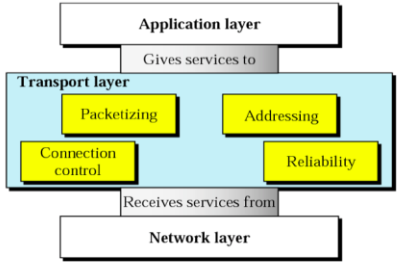
\includegraphics[width=0.7\linewidth]{chapters/8/images/trasporto.png}
\end{figure}

\noindent I due protocolli del livello di trasporto utilizzati in internet 
sono TCP e UDP.

\subsection{Porte}
Un numero di porta è un intero a 16 bit che assume un valore comprso 
tra 0 e 65535. I numeri di porta tra 0 e 1023 (i cosidetti \textit{numeri di
porta noti}) sono riservati ad applicazioni come HTTP, \dots

\section{TCP (Transmission Control Protocol)}
\begin{itemize}
    \item \textbf{Mittente:} suddivide i dati in pacchetti; ad ogni pacchetto è associato un numero di sequenza
    \item \textbf{Ricevitore:} riassembla i pacchetti nell'ordine corretto; i pacchetti persi vengono rispediti
\end{itemize}

\begin{figure}[H]
    \centering
    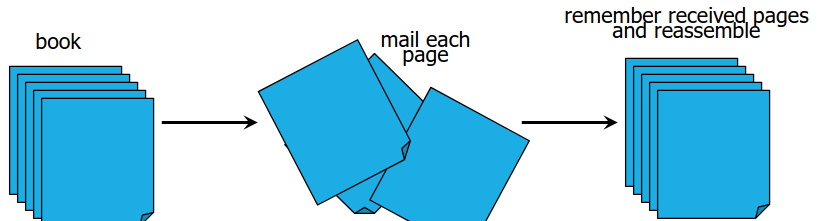
\includegraphics[width=1\linewidth]{chapters/8/images/tcp.png}
\end{figure}

\subsection{Flag TCP}
\begin{itemize}
    \item \textbf{SYN:} richiesta di connessione, primo pacchetto della comunicazione 
    \item \textbf{FIN:} intenzione del mittente di terminare la sessione
    \item \textbf{ACK:} conferma del pacchetto precedente
    \item \textbf{RST:} reset della sessione 
    \item \textbf{URG:} dati urgenti che vengono inviati con precedenza sugli altri (es. CTRL+C) 
\end{itemize}

\subsection{TCP handshake}
Le connessioni TCP vengono stabilite tramite un handshake a tre vie:
\begin{itemize}
    \item il server ha generalmente un listener passivo, in attesa di una richiesta di connessione 
    \item il client richiede una connessione inviando un pacchetto SYN 
    \item il server risponde inviando un pacchetto SYN/ACK, indicando un riconoscimento per la connessione 
    \item il client risponde inviando un ACK al server, stabilendo così la connessione
\end{itemize}

\begin{figure}[H]
    \centering
    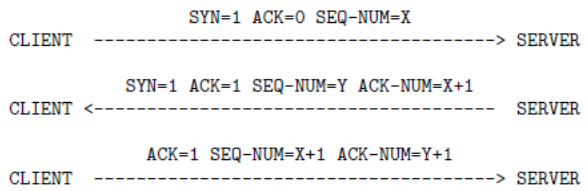
\includegraphics[width=0.8\linewidth]{chapters/8/images/tcp-handshake.png}
\end{figure}

\subsection{Problemi intrinsechi}
\begin{itemize}
    \item \textbf{Non c'è autenticazione} fra le parti; un utente malevolo potrebbe 
    intromettersi nella connessione fintanto che usa un \textit{sequence number} corretto 
    e gli indirizzi IP sono corretti 
    \item i \textbf{controlli di integrità} sono banali
\end{itemize}

\section{Spoofing}

\subsection{TCP spoofing}
Ogni connessione TCP ha uno stato associato:
\begin{itemize}
    \item numero di sequenza 
    \item numero di porta 
\end{itemize}

$\rightarrow$ è facile da indovinare, dato che si usano numeri di porta standard e numeri 
di sequenza prevedibili

\noindent È dunque possibile iniettare pacchetti in connessioni esistenti:
\begin{itemize}
    \item se l'attaccante conosce il numero di sequenza iniziale e la quantità di traffico, può indovinare 
    il probabile numero corrente 
    \item altrimenti, dato che la maggior parte dei sistemi accetta grandi finestre di numeri di sequenza per gestire 
    le perdite di pacchetti, invia un flusso di pacchetti con probabili numeri di sequenza
\end{itemize}